%*******************************************************************************
%****************************** Second Chapter *********************************
%*******************************************************************************

\chapter{Thiết kế và hiện thực \newline sản phẩm móc khóa thông minh - Smart Keyring}

\ifpdf
    \graphicspath{{Chapter2/Figs/Raster/}{Chapter2/Figs/PDF/}{Chapter2/Figs/}}
\else
    \graphicspath{{Chapter2/Figs/Vector/}{Chapter2/Figs/}}
\fi


%\section[Short title]{Reasonably long section title}
\section{Thiết kế sản phẩm}
% Uncomment this line, when you have siunitx package loaded.
%The SI Units for dynamic viscosity is \si{\newton\second\per\metre\squared}.
\textit{Thiết kế tính năng sản phẩm:}

\label{feature}
Sản phẩm Smart Keyring sẽ có các tính năng cơ bản như:

• Báo hiệu khi mất kết nối: hỗ trợ việc cảnh báo người tránh bỏ quên 1 trong 2 thiết bị.

• Báo hiệu khi kích hoạt chức năng tìm kiếm: cho phép người dùng định vị thiết bị còn lại trong phạm vi kết nối.

• Hai chế độ báo hiệu bằng âm thanh hoặc ánh sáng đèn led hoặc cả 2: mục đích sử dụng trong nhiều trường hợp khác nhau như đêm tối, không gian yên tĩnh...

\section{Sơ đồ hoạt động}
\subsection{Tổng quát}
Sơ đồ hoạt động tổng quát:

\begin{figure}[h]
	\centering    
	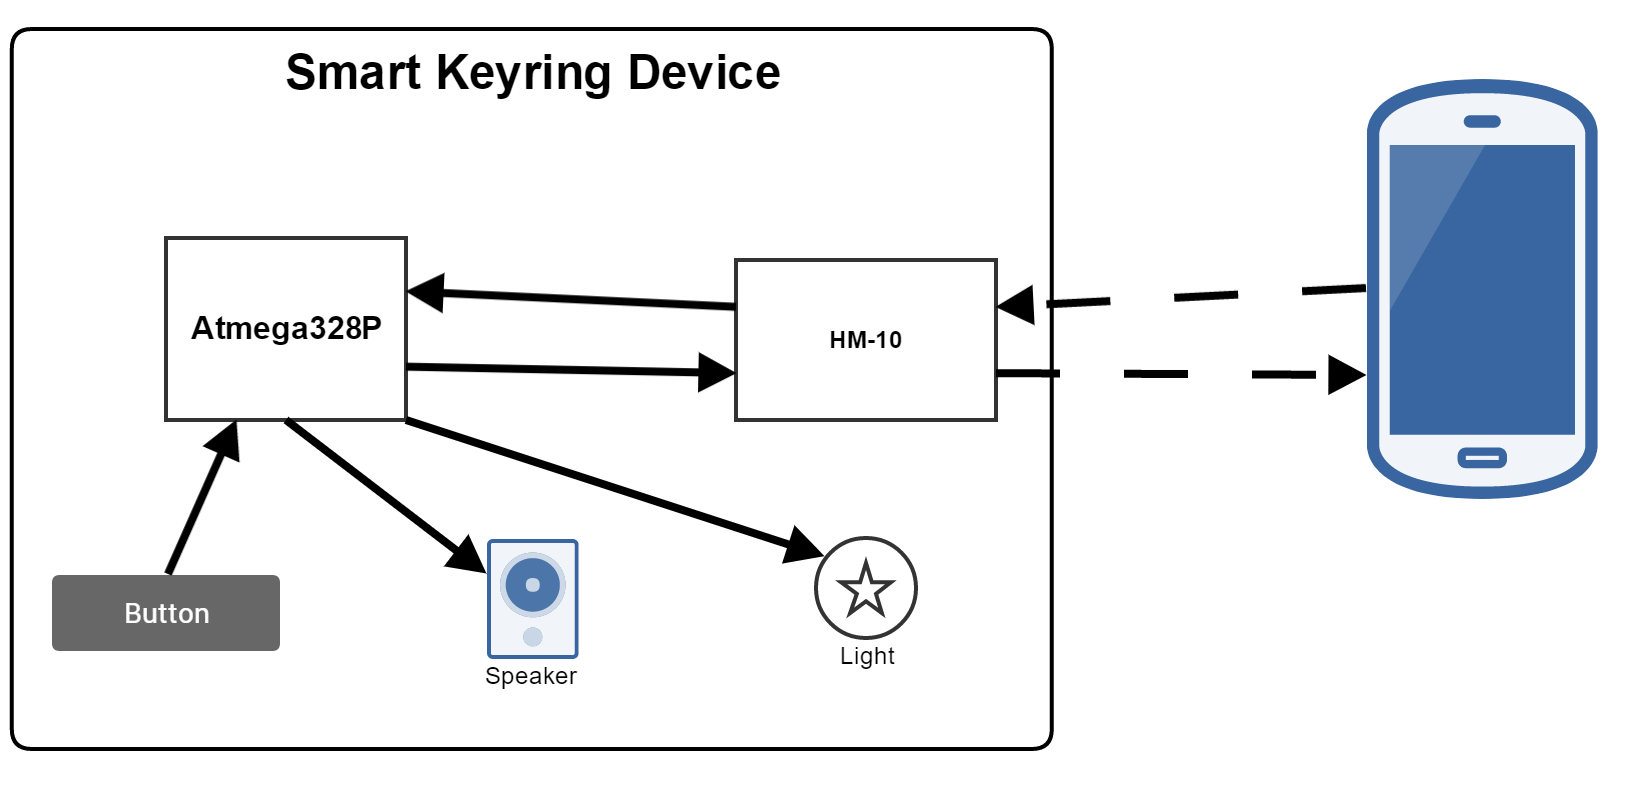
\includegraphics[width=1.0\textwidth]{general}
	\caption[Sơ đồ hoạt động tổng quát]{Sơ đồ hoạt động tổng quát}
	\label{fig: general}
\end{figure}

Như hình \ref{fig: general}, thiết bị Smart Keyring giao tiếp với thiết bị di động thông qua module BLE HM-10 và được điều khiển bởi MCU ATmega328P đảm nhận chức năng quản lý I/O như nút ấn, loa báo hiệu và đèn cũng như là truyền nhận thông điệp với module HM10.

\subsection{Nhận lệnh báo từ thiết bị di động}

Chức năng tìm kiếm thiết bị được kích hoạt bởi thiết bị di động được mô tả ở hình \ref{fig: ring1}.

Trình tự các hoạt động như sau:

(1) Thiết bị di động gửi gói tin với nội dung yêu cầu phát tín hiệu báo tới module HM-10.

(2) MCU ATmega328P nhận gói tin từ module HM-10 bằng giao thức UART với chế độ interrupt.

(3) Loa và đèn báo hiệu được kích hoạt tùy theo nội dung gói tin: kích hoạt cả hai hoặc chỉ kích hoạt đèn báo hiệu

(4*) Nút nhấn có chức năng ngắt chế độ báo hiệu khi cần thiết thông qua interrupt GPIO

\begin{figure}[h]
	\centering    
	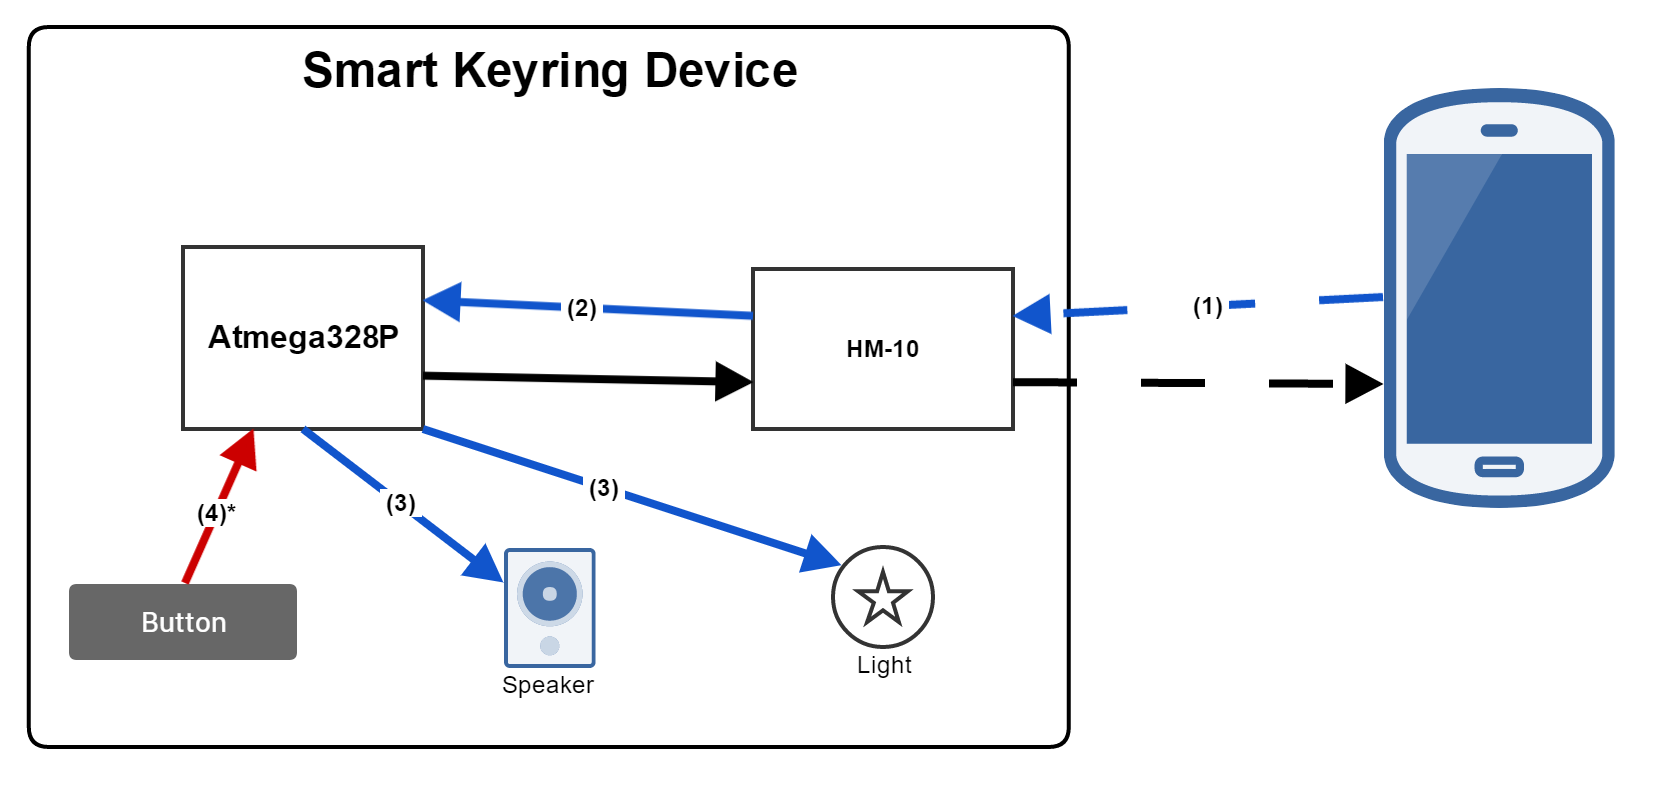
\includegraphics[width=1.0\textwidth]{ring1}
	\caption[Sơ đồ hoạt động khi nhận lệnh báo từ thiết bị di động]{Sơ đồ hoạt động khi nhận lệnh báo từ thiết bị di động}
	\label{fig: ring1}
\end{figure}

Sơ đồ hoạt động trên đúng với chức năng ngắt báo hiệu thiết bị được điều khiển bởi thiết bị di động, chỉ khác tại bước (3) là ngắt loa và đèn và không có bước (4).
\subsection{Kích hoạt thiết bị di động bật chế độ báo hiệu}

Chức năng kích hoạt thiết bị di động bật chế độ báo hiệu được mô tả ở hình \ref{fig: ring2}.

Trình từ các hoạt động như sau:

(1) MCU ATmega328P nhận tín hiệu điều khiển từ nút ấn thông qua interrupt GPIO

(2) Module BLE HM-10 nhận gói tin điều khiển từ MCU ATmega328 thông qua UART

(3) Thiết bị di động nhận gói tin truyền từ Module HM-10 và kích hoạt chế độ báo hiệu

\begin{figure}[h]
	\centering    
	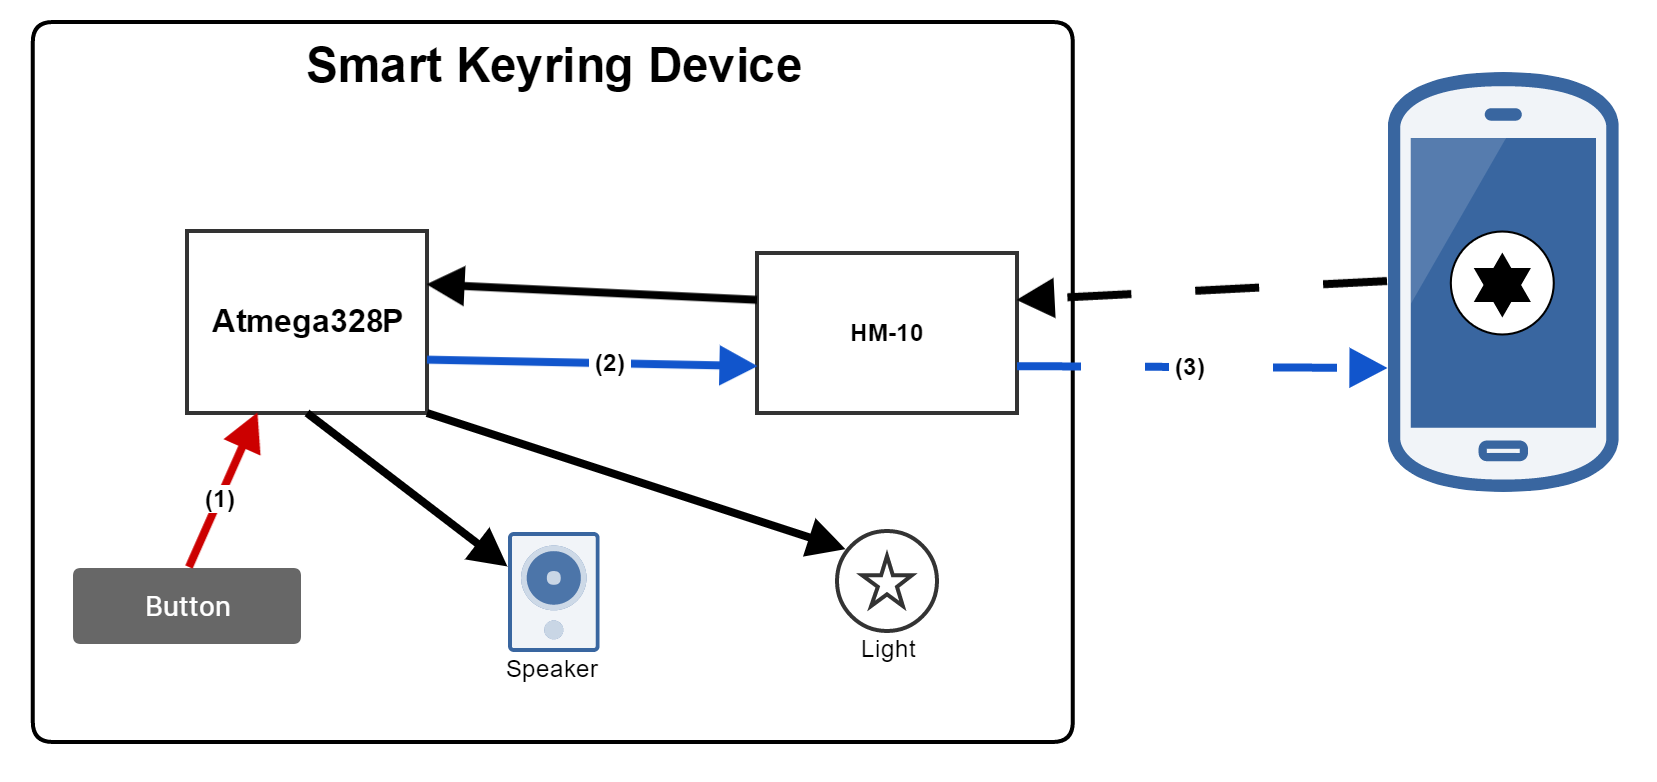
\includegraphics[width=1.0\textwidth]{ring2}
	\caption[Sơ đồ kích hoạt thiết bị di động bật chế độ báo hiệu]{Sơ đồ kích hoạt thiết bị di động bật chế độ báo hiệu}
	\label{fig: ring2}
\end{figure}
\newpage

\subsection{Sơ đồ trạng thái hoạt động khi ngắt kết nối}
Dựa theo tính năng sản phẩm ở mục \ref{feature}, sơ đồ trạng thái hoạt động được thiết kế ở hình \ref{fig: ble} và \ref{fig: blelost}

	\begin{figure}[h]
		\centering    
		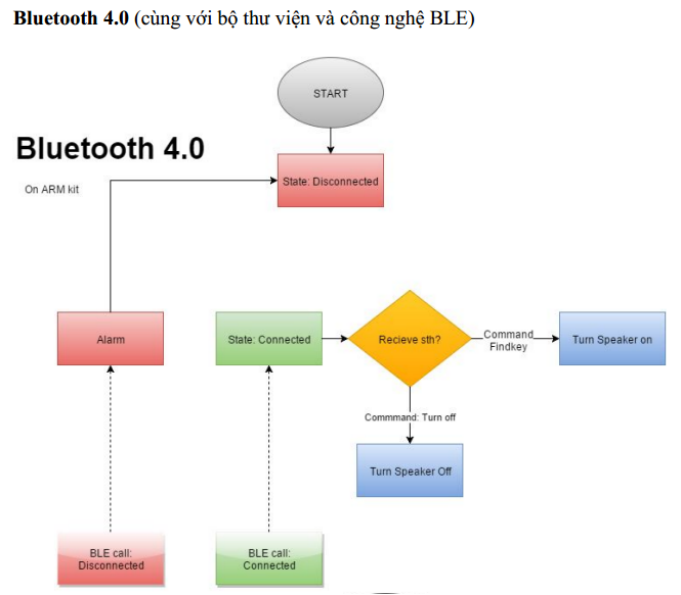
\includegraphics[width=1.0\textwidth]{ble}
		\caption[Sơ đồ trạng thái trên thiết bị Smart Keyring]{Sơ đồ trạng thái trên thiết bị Smart Keyring}
		\label{fig: ble}
	\end{figure}
	
	\begin{figure}[h]
		\centering    
		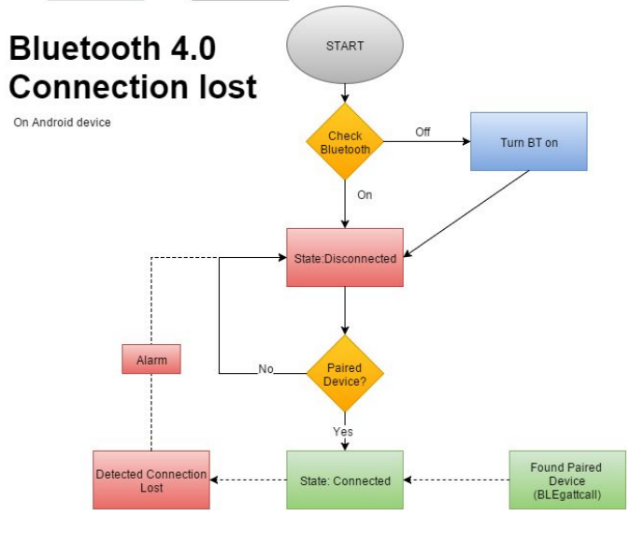
\includegraphics[width=1.0\textwidth]{blelost}
		\caption[Sơ đồ hoạt động trên thiết bị di động]{Sơ đồ hoạt động trên thiết bị di động}
		\label{fig: blelost}
	\end{figure}
\newpage
\section{Hiện thực phần cứng}
\subsection{Mô hình hoạt động}
Dựa theo tính năng sản phẩm ở mục \ref{feature}, mô hình ứng dụng khi bị thất lạc được thế kế như hình \ref{fig: ble}


\subsection{Hiện thực}
\newpage
\section{Hiện thực ứng dụng di động trên Android}
\subsection{Mô hình hoạt động}

\subsection{Các module trong ứng dụng Android}

